%!TEX root = ../clcxsj.tex

\chapter{平面坐标系统之间的转换}

在某些工程中,由于不知道新旧两种坐标系的建立方法或参数,因此无法用换带计算的方法
进行坐标转换。如果知道某些点在两个坐标系中的坐标值,我们就可以采用一些近似的转换方
法将其它的点也转换到新坐标系中,求出其坐标值。尤其对于较低等级的大量控制点来说,
采用这些近似方法,能够快速得到转换结果。

 \section{原理和数学模型}

\subsection{原理}
这些方法的实质是根据新旧网的重合点(又称为公共点)的坐标值之差,按一定的规律修正
旧网的各点坐标值,使旧网最恰当的配合到新网内。修正时因不合观测值改正数平方和为最
小的原则,故为近似方法。

\begin{figure}[htbp]
    \centering
    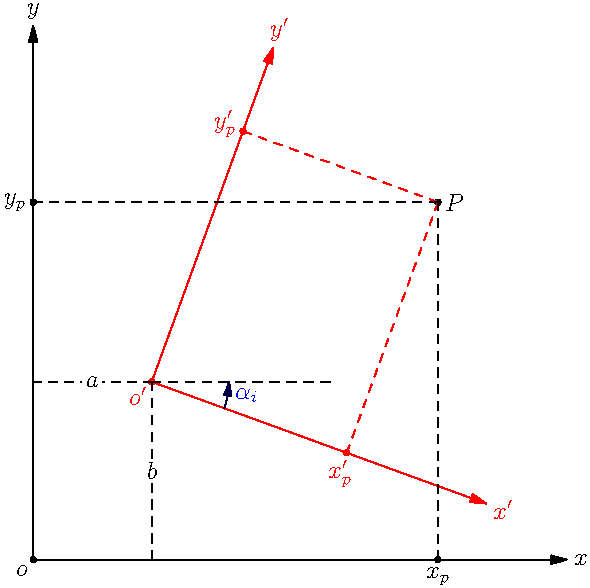
\includegraphics[scale=1]{xytoxy/xytoxy.pdf}
    \caption{坐标相似变换示意图}
    \label{fig:xytoxy}
\end{figure}

常用的方法有简单变换方法(又称赫尔默特法或相似变换法)、仿射变换法、正形变换法等。
在这里我们主要讲解简单变换法。

\subsection{相似变换法的数学模型}
实质是使旧网坐标系平移、旋转和进行尺度因子改正,将旧网配合到新网上。因旧网形状保
持不变,故称为平面相似变换法。

变换方程为:
$$\left.
\begin{array}{l}
\textrm{$x=dx + k(x'\cos\alpha - y'\sin\alpha)$} \\
\textrm{$y=dy + k(x'\sin\alpha + y'\cos\alpha)$} 
\end{array}\right\}$$

式中$a$,$b$表示平移,$\alpha$是旧网$x'$轴逆转至新网$x$轴的转角,$k$为尺度因子。
这些变换参数是未知的,要根据新旧网公共点上的已知坐标$x$,$y$和$x'$、$y'$求解确定。

因此必须至少有两个公共点,列出四个方程式,解算出这四个未知参数值。如果具有两个以
上的公共点时,就应该应用最小二乘平差方法,求解最或是参数值。

为解算出这些参数,我们引入参数$a$、$b$、$c$、$d$:

$a=dx, b=dy, c=k\cos\alpha, d=k\sin\alpha$

将公式转换为:
$$\left.
\begin{array}{l}
\textrm{$x = a + x'c - y'd$}\\
\textrm{$y = b + y'c + x'd$}
\end{array}\right\}$$

由于新旧网都存在测量误差,设新旧坐标$x$,$y$和$x'$,$y'$的误差分别为
$v_x$,$v_y$和$v_{x'}$,$v_{y'}$,因此上式改写为:

$$\left.\begin{array}{l}
\textrm{$x + v_x = a + (x'+v_{x'})c - (y'+v_{y'})d$} \\
\textrm{$y + v_y = b + (y'+v_{y'})c + (x'+v_{x'})d$}
\end{array}\right\}$$

设:
$$\left.\begin{array}{l}
\textrm{$n_x = -v_x + cv_{x'} - dv_{y'}$} \\
\textrm{$n_y = -v_y + cv_{y'} + dv_{x'}$}
\end{array}\right\}$$

则有:
$$\left.\begin{array}{l}
\textrm{$-n_x = a + x'c - y'd - x$} \\
\textrm{$-n_y = b + y'c + x'd - y$}
\end{array}\right\}$$

若有$r$个新旧网的公共点,则可组成$r$对方程:
$$V=BX-l$$

上式即为参数平差时的方程,$l$代表观测向量,$V$代表改正数向量,$B$代表系数矩阵,
$X$是参数向量。它们的值为:

$\mathbf{V}=
\left(\begin{array}{c}
-n_{x1} \\ -n_{y1} \\ \vdots \\ -n_{xr} \\ -n_{yr}
\end{array}\right)$
$\mathbf{B}=
\left(\begin{array}{cccc}
1 & 0 & x'_1 & -y'_1 \\
0 & 1 & y'_1 &  x'_1 \\
\dots & \dots & \ldots & \ldots \\
1 & 0 & x'_r & -y'_r \\
0 & 1 & y'_r &  x'_r
\end{array}\right)$
$\mathbf{X}=
\left(\begin{array}{c}
a \\ b \\ c \\ d
\end{array}\right)$
$\mathbf{l}=
\left(\begin{array}{c}
x_1 \\ y_1 \\ \vdots \\ x_r \\ y_r
\end{array}\right)$

根据最小二乘原理$V^TV=min$可得到法方程:
$$B^TBX-B^Tl=0$$

解法方程可求得$a$、$b$、$c$、$d$的值:
$$X=(B^TB)^{-1}(B^Tl)$$

旋转角$\alpha$和尺度比$k$为:
$$\alpha=\arctan\frac{d}{c}$$
$$k=\sqrt{c^2+d^2}$$
之后,就可计算旧网中所有待转换点的新坐标。

计算出系数$a,b,c,d$ 或 $dx, dy, k, \alpha$ 后可带入前面相应的公式
计算出其它点由源坐标系坐标转换到目标坐标系中的坐标。


\section{程序设计与实现}

程序整体功能比较单一,从数学模型分析可看出,程序的关
键是在于如何组成系数矩阵$B$与常数项$l$。

\subsection{程序功能分析}

在程序中,我们需要能够有录入数据界面手工输入数据,能够导入与导出
文本文件形式组织的数据,能够输出计算成果,能够计算转换系数或根据已有的
转换系数也能计算待计算点在新坐标系中的坐标。

由此,我们设计出程序界面如图\ref{fig:XYtoXYUI02}所示:

\begin{figure}[htbp]
    \centering
    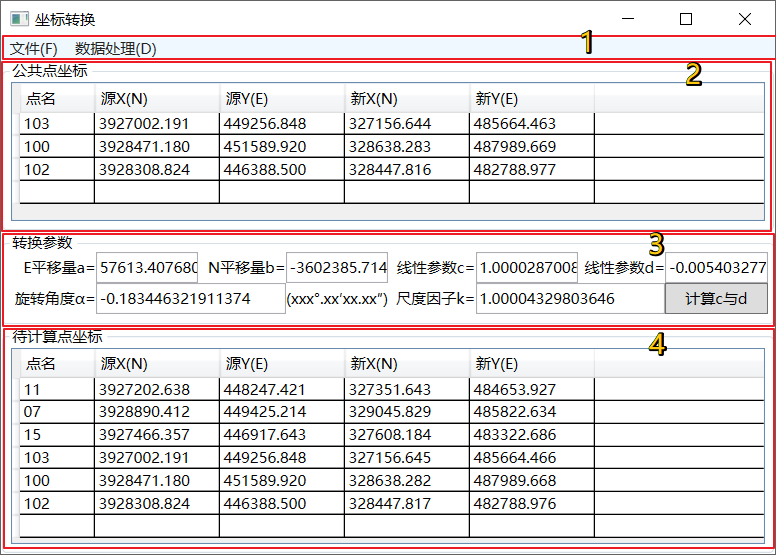
\includegraphics[scale=0.8]{xytoxy/XYtoXYUI02.png}
    \caption{坐标转换程序界面}
    \label{fig:XYtoXYUI02}
\end{figure}

\subsection{程序界面设计}

由图\ref{fig:XYtoXYUI02}分析可知,界面分为菜单、公共点坐标、转换参数与
待计算点坐标四个部分。

整个界面采用DockPanel布局,以加入菜单项,使用菜单项进行功能计算可以有效节省
界面的布局空间。余下的部分采用Grid布局,将其划分为三行,
即三个部分。第一行中加入GroupBox控件作为标题,在其中加入DataGrid控件;
第二部分中加入Grid布局,将其二行八列进行布局;第三部分同第一部分一样。

由于需要根据输入的a、b、$\alpha$、k计算各点在新坐标系中的坐标,为了输入
旋转角度的便捷性(直接输入度分秒),因此加入了计算c与d的按钮。程序中计算各待计算点坐标
时实际使用的参数是$a,b,c,d$。

整个界面布局xaml代码如下:
\begin{lstlisting}[language=xml]
<DockPanel LastChildFill="True">
    <Menu  x:Name="mainmenu" DockPanel.Dock="Top" Background="AliceBlue">
        <MenuItem Header="文件(F)">
            <MenuItem Header="打开文本数据"
               Click="menuItem_OpenTextFileData_Click"/>
            <MenuItem Header="保存文本数据"
                Click="menuItem_SaveTextFileData_Click"/>
            <Separator/>
            <MenuItem Header="退出" Click="menuItem_Exit_Click"/>
       </MenuItem>
        <MenuItem Header="数据处理(D)">
            <MenuItem Header="计算转换参数" 
                Click="menuItem_CalCoefficient_Click" />
            <MenuItem Header="计算待计算点坐标" 
                Click="menuItem_Cal_UnKnw_XY_Click" />
            <Separator/>
            <MenuItem Header="写出计算成果" 
                Click="menuItem_Write_Result_Click" />
        </MenuItem>
    </Menu>

    <Grid>
        <Grid.RowDefinitions>
            <RowDefinition Height="150*"/>
            <RowDefinition Height="75"/>
            <RowDefinition Height="200*"/>
        </Grid.RowDefinitions>
        <GroupBox Header="公共点坐标" Grid.Row="0">
        <DataGrid AutoGenerateColumns="False" Margin="2" 
            ItemsSource="{Binding KnwPointList}">
            <DataGrid.Columns>
                <DataGridTextColumn Header="点名" MinWidth="60"
                    Binding="{Binding Name}"  />
                <DataGridTextColumn Header="源X(N)" MinWidth="100"
                    Binding="{Binding OX, StringFormat={}{0:0.000}}"/>
                <DataGridTextColumn Header="源Y(E)" MinWidth="100"
                    Binding="{Binding OY, StringFormat={}{0:0.000}}"/>
                <DataGridTextColumn Header="新X(N)"  MinWidth="100"
                    Binding="{Binding NX, StringFormat={}{0:0.000}}"/>
                <DataGridTextColumn Header="新Y(E)" MinWidth="100"
                    Binding="{Binding NY, StringFormat={}{0:0.000}}"/>
            </DataGrid.Columns>
        </DataGrid>
            </GroupBox>

            <GroupBox Header="转换参数" Grid.Row="1">
                <Grid>
                    <Grid.ColumnDefinitions>
                        <ColumnDefinition Width="70"/>
                        <ColumnDefinition Width="120*"/>
                        <ColumnDefinition Width="70"/>
                        <ColumnDefinition Width="120*"/>
                        <ColumnDefinition Width="70"/>
                        <ColumnDefinition Width="120*"/>
                        <ColumnDefinition Width="70"/>
                        <ColumnDefinition Width="120*"/>
                    </Grid.ColumnDefinitions>
                    <Grid.RowDefinitions>
                        <RowDefinition Height="25"/>
                        <RowDefinition Height="25"/>
                    </Grid.RowDefinitions>
                    <TextBlock Text="E平移量a=" Grid.Row="0" Grid.Column="0" 
                        VerticalAlignment="Center" HorizontalAlignment="Right"/>
                    <TextBox x:Name="textBox_a" Grid.Row="0" Grid.Column="1" 
                        Text="{Binding a}" 
                        VerticalContentAlignment="Center"/>
                    <TextBlock Text="N平移量b=" Grid.Row="0" Grid.Column="2"  
                        VerticalAlignment="Center" HorizontalAlignment="Right"/>
                    <TextBox x:Name="textBox_b" Grid.Row="0" Grid.Column="3"  
                        Text="{Binding b}"
                        VerticalContentAlignment="Center"/>
                    <TextBlock Text="线性参数c=" Grid.Row="0" Grid.Column="4" 
                        VerticalAlignment="Center" HorizontalAlignment="Right"/>
                    <TextBox x:Name="textBox_c" Grid.Row="0" Grid.Column="5" 
                        Text="{Binding c}"
                        VerticalContentAlignment="Center"/>
                    <TextBlock Text="线性参数d=" Grid.Row="0" Grid.Column="6" 
                        VerticalAlignment="Center" HorizontalAlignment="Right"/>
                    <TextBox x:Name="textBox_d" Grid.Row="0" Grid.Column="7"  
                        Text="{Binding d}" 
                        VerticalContentAlignment="Center"/>
                    <TextBlock Text="旋转角度α=" Grid.Row="1" Grid.Column="0" 
                        VerticalAlignment="Center" HorizontalAlignment="Right"/>
                    <TextBox x:Name="textBox_alpha" Grid.Row="1" Grid.Column="1"  
                        Text="{Binding alpha}" 
                        Grid.ColumnSpan="2"
                        VerticalContentAlignment="Center"/>
                    <TextBlock Text="(xxx°.xx′xx.xx″)" Grid.Row="1" Grid.Column="3" 
                        VerticalAlignment="Center" HorizontalAlignment="Right"/>
                    <TextBlock Text="尺度因子k=" Grid.Row="1" Grid.Column="4" 
                        VerticalAlignment="Center" HorizontalAlignment="Right"/>
                    <TextBox x:Name="textBox_k" Grid.Row="1" Grid.Column="5" 
                        Text="{Binding k}" 
                        Grid.ColumnSpan="2"
                        VerticalContentAlignment="Center"/>
                    <Button x:Name="button_Cal_cd"  Content="计算c与d"
                        Grid.Row="1" Grid.Column="7" 
                        Click="button_Cal_cd_Click"/>
                </Grid>
            </GroupBox>

            <GroupBox Header="待计算点坐标" Grid.Row="2">
                <DataGrid AutoGenerateColumns="False" Margin="2" 
                    ItemsSource="{Binding UnKnwPointList}">
                    <DataGrid.Columns>
                        <DataGridTextColumn Header="点名" MinWidth="60"
                            Binding="{Binding Name}"  />
                        <DataGridTextColumn Header="源X(N)"  MinWidth="100"
                            Binding="{Binding OX, StringFormat={}{0:0.000}}"/>
                        <DataGridTextColumn Header="源Y(E)" MinWidth="100"
                            Binding="{Binding OY, StringFormat={}{0:0.000}}"/>
                        <DataGridTextColumn Header="新X(N)" MinWidth="100"
                            Binding="{Binding NX,StringFormat={}{0:0.000}}" />
                        <DataGridTextColumn Header="新Y(E)" MinWidth="100"
                            Binding="{Binding NY, StringFormat={}{0:0.000}}" />
                    </DataGrid.Columns>
                </DataGrid>
            </GroupBox>
        </Grid>
    </DockPanel>
\end{lstlisting}

\subsection{数据文件和成果文件格式}
由于程序的功能较为单一,数据文件的格式也较为简单。我们设计格式如下:
\begin{verbatim}
#赫尔默特四参数转换法数据文件
#每行以“#”开头的行均被认为是注释行
#公共点在源坐标系中的坐标: 点名, X(N), Y(E)
103, 3927002.191, 449256.848
100, 3928471.180, 451589.920
102, 3928308.824, 446388.500

#公共点在目标坐标系中的坐标: 点名, X(N), Y(E)
102, 328447.816, 482788.977
103, 327156.644, 485664.463
100, 328638.283, 487989.669

#待转换点在源坐标系中的坐标: 点名, X(N), Y(E)
11,   3927202.638, 448247.421
07,   3928890.412, 449425.214
15,   3927466.357, 446917.643
103, 3927002.191, 449256.848
100, 3928471.180, 451589.920
102, 3928308.824, 446388.500
\end{verbatim}

我们设计成果文件的格式如下:

\begin{lstlisting}[language=C]
#赫尔默特四参数转换法计算成果数据文件
# 公共点坐标
# 点名, 源X(N), 源Y(E), 新X(N), 新Y(E)
103,3927002.191,449256.848,327156.644,485664.463
100,3928471.180,451589.920,328638.283,487989.669
102,3928308.824,446388.500,328447.816,482788.977

# 转换参数
a=57613.4076806228,b=-3602385.71435623, c=1.00002870085641,
d=-0.00540327780963763
`$\alpha$`=-0.183446321911374,k=1.00004329803646

# 待计算点的坐标
# 点名, 源X(N), 源Y(E), 新X(N), 新Y(E)
11,3927202.638,448247.421,327351.643,484653.927
07,3928890.412,449425.214,329045.829,485822.634
15,3927466.357,446917.643,327608.184,483322.686
103,3927002.191,449256.848,327156.645,485664.466
100,3928471.180,451589.920,328638.282,487989.668
102,3928308.824,446388.500,328447.817,482788.976
\end{lstlisting}

\subsection{程序流程}
根据以上分析,程序流程如下:
\begin{enumerate}
  \item 读取公共点旧坐标
  \item 读取公共点新坐标
  \item 组成误差方程式
  \item 解算参数向量
  \item 解算待定点的坐标
  \item 将计算成果写入文件
\end{enumerate}


\subsection{主要功能设计}
为了实现以上功能,我们需要设计一个类(或结构)用于表示点,设计如下:
\begin{lstlisting}[language=C]
namespace CoordniateTransform
{
    public class GeoPoint : NotificationObject
    {
        private string _name;
        public string Name //点名
        {
            get { return _name; }
            set
            {
                _name = value;
                RaisePropertyChange("Name");
            }
        }       

        private double _oX;
        public double OX //源X坐标
        {
            get { return _oX; }
            set
            {
                _oX = value;
                RaisePropertyChange("OX");
            }
        }
  
        private double _oY;
        public double OY  //源Y坐标
        {
            get { return _oY; }
            set
            {
                _oY = value;
                RaisePropertyChange("OY");
            }
        }


        private double _nX;
        public double NX //新X坐标
        {
            get { return _nX; }
            set
            {
                _nX = value;
                RaisePropertyChange("NX");
            }
        }

        private double _nY;
        public double NY  //新Y坐标
        {
            get { return _nY; }
            set
            {
                _nY = value;
                RaisePropertyChange("NY");
            }
        }

 
        public override string ToString()
        {
            return string.Format("{0},{1:0.000},{2:0.000},{3:0.000},{4:0.000}", Name, OX, OY, NX, NY);
        }
    }
}
\end{lstlisting}

类NotificationObject的设计见前一章内容。


同时,我们设计另一个类CoordinateSystem来完成相应的其它功能, 这个类相当于一个容器一样,
它包括点集(已知公共点集和待计算点集)、转换参数等,具体代码如下:

\begin{lstlisting}[language=C]
using System;
using System.Collections.ObjectModel;

namespace CoordniateTransform
{
    /// <summary>
    /// 坐标系
    /// </summary>
    public class CoordinateSystem : NotificationObject
    {
        /// <summary>
        /// 公共点集
        /// </summary>
        private ObservableCollection<GeoPoint> knwPointList = 
                new ObservableCollection<GeoPoint>();

        /// <summary>
        /// 公共点集
        /// </summary>
        public ObservableCollection<GeoPoint> KnwPointList
        {
            get { return knwPointList; }
        }
        
        /// <summary>
        /// 待计算点集
        /// </summary>
        private ObservableCollection<GeoPoint> unKnwPointList = 
                new ObservableCollection<GeoPoint>();

        /// <summary>
        ///待计算点集
        /// </summary>
        public ObservableCollection<GeoPoint> UnKnwPointList
        {
            get { return unKnwPointList; }
        }

        /// <summary>
        ///X方向平移量
        /// </summary>
        private double _a;

        /// <summary>
        /// X方向平移量
        /// </summary>
        public double a
        {
            get { return _a; }
            set
            {
                _a = value;
                RaisePropertyChange("a");
            }
        }

        /// <summary>
        /// Y方向平移量
        /// </summary>
        private double _b;

        /// <summary>
        /// Y方向平移量
        /// </summary>
        public double b
        {
            get { return _b; }
            set
            {
                _b = value;
                RaisePropertyChange("b");
            }
        }

        /// <summary>
        /// 线性方程计算系数c
        /// </summary>
        public double _c;

        /// <summary>
        /// 线性方程计算系数c
        /// </summary>
        public double c
        {
            get { return _c; }
            set
            {
                _c = value;
                RaisePropertyChange("c");
            }
        }

        /// <summary>
        /// 线性方程计算系数d
        /// </summary>
        public double _d;

        /// <summary>
        /// 线性方程计算系数d
        /// </summary>
        public double d
        {
            get { return _d; }
            set
            {
                _d = value;
                RaisePropertyChange("d");
            }
        }

        /// <summary>
        /// 旋转角度α
        /// </summary>
        public double _alpha;

        /// <summary>
        ///  旋转角度α
        /// </summary>
        public double alpha
        {
            get { return _alpha; }
            set
            {
                _alpha = value;
                RaisePropertyChange("alpha");
            }
        }

        /// <summary>
        /// 尺度比因子k
        /// </summary>
        public double _k;

        /// <summary>
        ///  尺度比因子k
        /// </summary>
        public double k
        {
            get { return _k; }
            set
            {
                _k = value;
                RaisePropertyChange("k");
            }
        }

        public CoordinateSystem(){ }

        /// <summary>
        /// 读入坐标转换数据文件
        /// </summary>
        /// <param name="fileName">文件名</param>
        public void ReadTextFileData(string fileName)
        {
            using (System.IO.StreamReader sr = new System.IO.StreamReader(fileName))
            {
                string buffer;

                //读入点的坐标数据
                this.KnwPointList.Clear();
                while (true)//读入公共点源坐标系坐标数据,至空行退出
                {
                    buffer = sr.ReadLine();
                    if (string.IsNullOrEmpty(buffer)) break; //文件末尾或空行退出

                    if (buffer[0] == '#') continue;

                    string[] its = buffer.Split(new char[1] { ',' });
                    if (its.Length == 3)
                    {
                        GeoPoint pnt = new GeoPoint();
                        pnt.Name = its[0].Trim();
                        pnt.OX = double.Parse(its[1]);
                        pnt.OY = double.Parse(its[2]);
                        this.KnwPointList.Add(pnt);
                    }
                }

                while (true)//读入公共点新坐标系坐标数据,至空行退出
                {
                    buffer = sr.ReadLine();
                    if (string.IsNullOrEmpty(buffer)) break; //文件末尾或空行退出

                    if (buffer[0] == '#') continue;

                    string[] its = buffer.Split(new char[1] { ',' });
                    if (its.Length == 3)
                    {
                        string name = its[0].Trim();
                        GeoPoint pnt = GetGeoPoint(name);
                        pnt.NX = double.Parse(its[1]);
                        pnt.NY = double.Parse(its[2]);
                    }
                }

                this.UnKnwPointList.Clear();
                while (true)//读入待计算点源坐标系坐标数据,至空行退出
                {
                    buffer = sr.ReadLine();
                    if (string.IsNullOrEmpty(buffer)) break; //文件末尾或空行退出

                    if (buffer[0] == '#') continue;

                    string[] its = buffer.Split(new char[1] { ',' });
                    if (its.Length == 3)
                    {
                        GeoPoint pnt = new GeoPoint();
                        pnt.Name = its[0].Trim();
                        pnt.OX = double.Parse(its[1]);
                        pnt.OY = double.Parse(its[2]);

                        this.UnKnwPointList.Add(pnt);
                    }
                }
            }
        }
     
        /// <summary>
        /// 根据点名获取点对象
        /// </summary>
        /// <param name="name">点名</param>
        /// <returns>点对象</returns>
        private GeoPoint GetGeoPoint(string name)
        {
            foreach (var it in this.KnwPointList)
            {
                if (it.Name == name)
                    return it;
            }

            return null;
        }

        /// <summary>
        /// 写坐标转换数据文件
        /// </summary>
        /// <param name="fileName">文件名</param>
        public void WriteTextFileData(string fileName)
        {
            using (System.IO.StreamWriter sr = new System.IO.StreamWriter(fileName))
            {
                sr.WriteLine("#赫尔默特四参数转换法数据文件");
                sr.WriteLine("#每行以“#”开头的行均被认为是注释行");
                sr.WriteLine("#公共点在源坐标系中的坐标: 点名, X(N), Y(E)");
                foreach (var pnt in this.knwPointList)
                {
                    sr.WriteLine("{0}, {1}, {2}", pnt.Name, pnt.OX, pnt.OY);
                }

                sr.WriteLine();
                sr.WriteLine("#公共点在新坐标系中的坐标: 点名, X(N), Y(E)");
                foreach (var pnt in this.knwPointList)
                {
                    sr.WriteLine("{0}, {1}, {2}", pnt.Name, pnt.NX, pnt.NY);
                }

                sr.WriteLine();
                sr.WriteLine("#待转换点在源坐标系中的坐标: 点名, X(N), Y(E)");
                foreach (var pnt in this.unKnwPointList)
                {
                    sr.WriteLine("{0}, {1}, {2}", pnt.Name, pnt.OX, pnt.OY);
                }
            }
        }
        /// <summary>
        /// 写计算成果数据文件
        /// </summary>
        /// <param name="fileName">文件名</param>
        public void WriteResultTextFileData(string fileName)
        {
            using (System.IO.StreamWriter sr = new System.IO.StreamWriter(fileName))
            {
                sr.WriteLine("#赫尔默特四参数转换法计算成果数据文件");
                sr.WriteLine("# 公共点坐标");
                sr.WriteLine("# 点名, 源X(N), 源Y(E), 新X(N), 新Y(E)");
                foreach (var pnt in this.knwPointList)
                {
                    sr.WriteLine(pnt);
                }

                sr.WriteLine();
                sr.WriteLine("# 转换参数");
                sr.WriteLine("a={0},b={1}, c={2}, d={3}\r\nα={4},k={5}", 
                    this.a, this.b, this.c, this.d, this.alpha, this.k);

                sr.WriteLine();
                sr.WriteLine("# 待计算点的坐标");
                sr.WriteLine("# 点名, 源X(N), 源Y(E), 新X(N), 新Y(E)");
                foreach (var pnt in this.unKnwPointList)
                {
                    sr.WriteLine(pnt);
                }
            }
        }

        /// <summary>
        /// 根据尺度比因子d与旋转角度α计算线性计算量c和d
        /// </summary>
        public void CalCd()
        {
            this.c = this.k * Math.Cos(ZXY.SMath.DMS2RAD(this.alpha));
            this.d = this.k * Math.Sin(ZXY.SMath.DMS2RAD(this.alpha));
        }

        /// <summary>
        /// 赫尔默特法计算转换系数
        /// </summary>
        public void CalCoefficient()
        {
            int n0 = this.knwPointList.Count;
            if (n0 < 2) return; //少于两个公共点,无法计算

            double[,] B = new double[2 * n0, 4];
            double[] l = new double[2 * n0];
            double[,] N = new double[4, 4];
            double[] U = new double[4];

            //组成系数阵B与l,此处应注意读入的坐标是测量坐标,
            //应将测量坐标转换为数学坐标
            double x, y, xT, yT;
            for (int i = 0; i < n0; i++)
            {
                x = knwPointList[i].OY;//数学上的x,测量上的y
                y = knwPointList[i].OX;//数学上的y,测量上的x
                xT = knwPointList[i].NY;
                yT = knwPointList[i].NX; 

                B[(2 * i), 0] = 1.0;
                B[(2 * i), 1] = 0.0;
                B[(2 * i), 2] = x;
                B[(2 * i), 3] = y;
                l[2 * i] = xT;

                B[(2 * i + 1), 0] = 0.0;
                B[(2 * i + 1), 1] = 1.0;
                B[(2 * i + 1), 2] = y; 
                B[(2 * i + 1), 3] = -x; 
                l[2 * i + 1] = yT;
            }

            for (int k = 0; k < 4; k++)
            {
                for (int j = 0; j < 4; j++)
                {
                    N[k, j] = 0.0;
                    for (int i = 0; i < 2 * n0; i++)
                    {
                        N[k, j] += B[i, k] * B[i, j];
                    }
                }

                U[k] = 0.0;
                for (int i = 0; i < 2 * n0; i++)
                    U[k] += B[i, k] * l[i];
            }

            NegativeMatrix(N, U, 4);

            this.a = U[0];
            this.b = U[1];
            this.c = U[2];
            this.d = U[3];
            this.alpha = ZXY.SMath.RAD2DMS(Math.Atan2(d, c));
            this.k = Math.Sqrt(d * d + c * c);
        }

        /// <summary>
        /// 计算点在新坐标系中的坐标
        /// </summary>
        public void CalUnKnwXY()
        {
            //应将测量坐标转换为数学坐标
            double x, y, xT, yT;
            foreach (var it in this.unKnwPointList)
            {
                x = it.OY; y = it.OX;

                xT = this.a + this.c * x + this.d * y;
                yT = this.b + this.c * y - this.d * x;

                it.NY = xT; it.NX = yT;
            }
        }

        /// <summary>
        ///  高斯约化法解方程 AX = B中的X值, 结果存B中
        /// </summary>
        /// <param name="A">A: nxn</param>
        /// <param name="B">B: nx1</param>
        /// <param name="n">n</param>
        private void NegativeMatrix(double[,] A, double[] B, int n)
        {
            for (int k = 0; k < n - 1; k++)
            {
                for (int i = k + 1; i < n; i++)
                {
                    A[i, k] /= A[k, k];
                    for (int j = k + 1; j < n; j++)
                    {
                        A[i, j] -= A[i, k] * A[k, j];
                    }
                    B[i] -= A[i, k] * B[k];
                }
            }
            B[n - 1] /= A[(n - 1), (n - 1)];
            for (int i = n - 2; i >= 0; i--)
            {
                double s = 0.0;
                for (int j = i + 1; j < n; j++)
                {
                    s += A[i, j] * B[j];
                }
                B[i] = (B[i] - s) / A[i, i];
            }
        }
    }
}
\end{lstlisting}

界面响应代码如下:

\begin{lstlisting}[language=C]
using Microsoft.Win32;
using System;
using System.Collections.Generic;
using System.Linq;
using System.Text;
using System.Threading.Tasks;
using System.Windows;
using System.Windows.Controls;
using System.Windows.Data;
using System.Windows.Documents;
using System.Windows.Input;
using System.Windows.Media;
using System.Windows.Media.Imaging;
using System.Windows.Navigation;
using System.Windows.Shapes;

namespace CoordniateTransform
{
    /// <summary>
    /// MainWindow.xaml 的交互逻辑
    /// </summary>
    public partial class MainWindow : Window
    {
        private CoordinateSystem cs;
        public MainWindow()
        {
            InitializeComponent();

            cs = new CoordinateSystem();
            this.DataContext = cs;
        }

        private void menuItem_OpenTextFileData_Click(object sender, RoutedEventArgs e)
        {
            OpenFileDialog dlg = new OpenFileDialog();
            dlg.DefaultExt = ".txt";
            dlg.Filter = "平面坐标相似变换数据文件|*.txt|All File(*.*)|*.*";
            if (dlg.ShowDialog() != true) return;

            cs.ReadTextFileData(dlg.FileName);
        }

        private void menuItem_SaveTextFileData_Click(object sender, RoutedEventArgs e)
        {
            SaveFileDialog dlg = new SaveFileDialog();
            dlg.DefaultExt = ".txt";
            dlg.Filter = "平面坐标相似变换数据文件|*.txt|All File(*.*)|*.*";
            if (dlg.ShowDialog() != true) return;

            cs.WriteTextFileData(dlg.FileName);
        }

        private void menuItem_CalCoefficient_Click(object sender, RoutedEventArgs e)
        {
            cs.CalCoefficient();
        }

        private void menuItem_Cal_UnKnw_XY_Click(object sender, RoutedEventArgs e)
        {
            cs.CalUnKnwXY();
        }

        private void menuItem_Write_Result_Click(object sender, RoutedEventArgs e)
        {
            SaveFileDialog dlg = new SaveFileDialog();
            dlg.DefaultExt = ".txt";
            dlg.Filter = "平面坐标相似变换成果数据文件|*.txt|All File(*.*)|*.*";
            if (dlg.ShowDialog() != true) return;

            cs.WriteResultTextFileData(dlg.FileName);
        }

        private void menuItem_Exit_Click(object sender, RoutedEventArgs e)
        {
            this.Close();
        }

        private void button_Cal_cd_Click(object sender, RoutedEventArgs e)
        {
            cs.CalCd();
        }
    }
}
\end{lstlisting}



%%TODO
%%以上方法容易产生病态矩阵,导致计算出的结果与参数不争取
%%本人设想:
%%根据新旧坐标系统的已知公共点,求出其中心坐标点,
%%将数据规化后再组成 系数阵、法方程 进行计算
%%此处教材中应该改写这部分内容与程序

\section{算法与程序的优化}
在上面的计算中,由于误差方程$V=BX-l$中的系数阵B中直接是由点的坐标X、Y组成的,
而一般X、Y的数值都比较大,非常容易形成病态矩阵,从而导致法方程N中的数值更大,
在计算系数阵X时得不到正确的结果。

变换方程为:
$$\left.
\begin{array}{l}
\textrm{$x-kx =dx + k[(x'-kx') \cos\alpha - (y'-ky') \sin\alpha]$} \\
\textrm{$y-ky =dy + k[(x'-kx') \sin\alpha + (y'-ky') \cos\alpha]$} 
\end{array}
\right\}$$


将公式做一变换:
令 $DX = dx+kx, DY=dy+ky, X'=x'-kx', Y'=y'-ky'$

则上式变为:

$$\left.
\begin{array}{l}
\textrm{$x =DX + k[X' \cos\alpha - Y' \sin\alpha]$} \\
\textrm{$y =DY + k[X' \sin\alpha + Y' \cos\alpha]$} 
\end{array}
\right\}$$

则该算法与前边算法没有本质上的区别,但可以将公式中的X、Y坐标中的大数值变小。

